\chapter{PERFIL DE COOPERAÇÃO PREDITIVA: OBJETOS FORMAIS E INDICADORES DE PRESERVAÇÃO}
\label{chap:metricas}

\section{Da perda média estimada ao perfil de cooperação preditiva}

A perda média definida na Equação \eqref{eq:mean-loss} é a matéria-prima do estudo, mas o objeto científico não se reduz ao menor valor absoluto de erro. Para cada braço, classificador e tamanho amostral, as perdas médias estimadas induzem o \PredictiveCooperationProfile{}, organizado em três níveis analíticos de detalhe crescente: a \textbf{ordenação global} dos subconjuntos em cada $n$ (Seção~\ref{sec:ranking}); a \textbf{relação efetiva de vencedor} par a par, representada pela matriz $\Wmat(n)$, com uma regra explícita de propagação sob empate exato (Seções~\ref{sec:winner-relation}--\ref{sec:winner-agreement}); e a \textbf{dinâmica de inversões}, representada pela matriz triangular $\Rmat(n_t)$, que produz dois indicadores de preservação logicamente distintos --- existência (Seção~\ref{sec:ar}) e regime amostral (Seção~\ref{sec:sr}) --- nunca combinados em um único índice.

Os relatórios de simulação disponibilizam todas as curvas, rankings e matrizes; o PDF emprega apenas exemplos selecionados, pois reproduzir cada objeto para 31 ou 127 subconjuntos em todos os braços e classificadores impediria a leitura da argumentação principal. As definições auxiliares mais extensas --- casos de empate, conjuntos de eventos de inversão e exemplos didáticos completos --- são apresentadas no Apêndice~D. A Figura~\ref{fig:conceito-metricas} antecipa, em um exemplo esquemático, os três níveis analíticos que este capítulo formaliza.

\begin{figure}[H]
  \centering
  \caption{Visão esquemática dos três níveis analíticos do perfil de cooperação preditiva}
  \label{fig:conceito-metricas}
  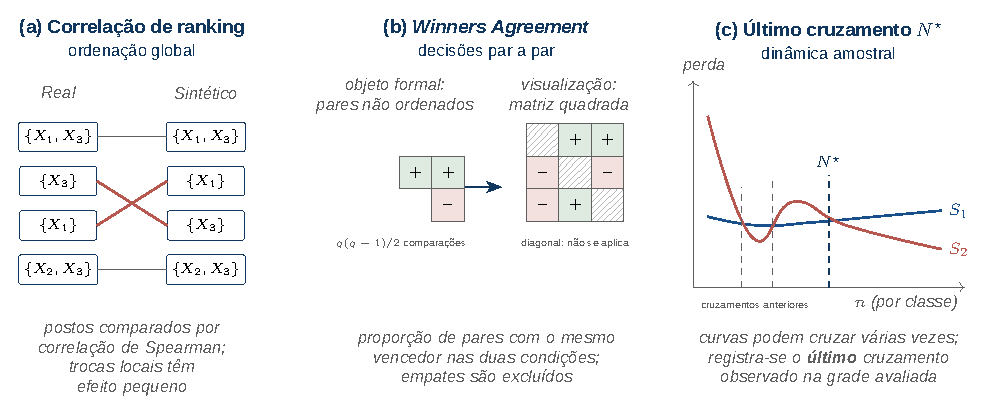
\includegraphics[width=\textwidth]{figures/conceptual/metricas_tres_paineis.pdf}
  \sourcebelow{elaboração própria}
  \notailustracao{No painel (b), o objeto formal armazena apenas os pares não ordenados; a matriz quadrada exibida nos relatórios é uma visualização redundante. No painel (c), $A_R$ e $S_R$ são construídos separadamente e nunca multiplicados}
\end{figure}

\section{Ordenação dos subconjuntos e correlação de ranking}
\label{sec:ranking}

Sejam $q=|\mathcal{S}|$ subconjuntos em uma ordem canônica. Para um braço $g$, classificador $f$ e tamanho $n$, o vetor de perdas médias estimadas é
\begin{equation}
  \bm\ell^{(g,f)}(n)=
  \left(
    \overline{L}^{(g)}_{S_1,f}(n),\ldots,
    \overline{L}^{(g)}_{S_q,f}(n)
  \right).
\end{equation}
O vetor de postos $\bm r^{(g,f)}(n)$ atribui posto 1 à menor perda e utiliza o posto médio em empates exatos. O ranking completo permite observar não apenas qual subconjunto aparece primeiro, mas se grupos de alternativas permanecem próximos e se configurações menores conservam vantagem sobre configurações mais caras.

A correlação de ranking entre um braço sintético $g$ e o braço real de referência $R$ é a correlação de Spearman \cite{spearman1904}:
\begin{equation}
  \rankrho^{(g,f)}(n)
  =\operatorname{corr}_{\mathrm{Spearman}}
  \left(\bm r^{(R,f)}(n),\bm r^{(g,f)}(n)\right).
  \label{eq:rank-rho}
\end{equation}
Valores próximos de 1 indicam ordenações semelhantes; valores próximos de 0 indicam ausência de associação monotônica; valores negativos representam inversão ampla. Quando um dos rankings é constante, a correlação não é definida; a autocorrelação do braço de referência é fixada em 1.

A medida é global: uma troca entre dois subconjuntos quase empatados pode ter efeito pequeno em $\rankrho$, enquanto muitas trocas reduzem a correlação. Essa propriedade é desejável para planejamento operacional, pois não transforma automaticamente uma diferença mínima no primeiro lugar em falha de preservação total. Por descrever apenas a ordenação, $\rankrho$ não distingue, por si só, \emph{qual} par mudou de vencedor nem \emph{quando} --- essas perguntas são respondidas pelos objetos das seções seguintes.

\section{Relação efetiva de vencedor e matriz de vencedores \texorpdfstring{$\Wmat$}{W}}
\label{sec:winner-relation}

Para dois subconjuntos $S_i$ e $S_j$ ($i<j$), o resultado par a par observado em $n_k$ é
\begin{equation}
  U^{(g,f)}_{ij}(n_k)=
  \begin{cases}
    +1, & \overline{L}^{(g)}_{S_i,f}(n_k)<\overline{L}^{(g)}_{S_j,f}(n_k),\\
    -1, & \overline{L}^{(g)}_{S_i,f}(n_k)>\overline{L}^{(g)}_{S_j,f}(n_k),\\
    0,  & \overline{L}^{(g)}_{S_i,f}(n_k)=\overline{L}^{(g)}_{S_j,f}(n_k),
  \end{cases}
  \label{eq:observed-outcome}
\end{equation}
com $+1$ indicando que $S_i$ tem menor perda, $-1$ que $S_j$ tem menor perda, e $0$ um empate exato observado naquele ponto da grade.

Um resultado observado isolado, porém, não é uma boa base para comparar braços ao longo de $n$: um empate exato --- comum quando duas curvas se cruzam exatamente sobre um ponto da grade --- não deveria apagar o vencedor já estabelecido no ponto anterior. Por isso, define-se a \textbf{relação efetiva de vencedor} $\Wmat$ por propagação determinística:
\begin{equation}
  W^{(g,f)}_{ij}(n_k)=
  \begin{cases}
    U^{(g,f)}_{ij}(n_k), & U^{(g,f)}_{ij}(n_k)\neq0,\\[2pt]
    W^{(g,f)}_{ij}(n_{k-1}), & U^{(g,f)}_{ij}(n_k)=0 \text{ e existe vencedor anterior},\\[2pt]
    0, & U^{(g,f)}_{ij}(n_k)=0 \text{ e não existe vencedor anterior}.
  \end{cases}
  \label{eq:winner-relation}
\end{equation}
A regra tem quatro consequências diretas, usadas em todo o restante deste capítulo: empates exatos iniciais permanecem indefinidos ($W=0$); o primeiro vencedor estrito inicializa a relação; um empate exato posterior \textbf{mantém} o vencedor efetivo anterior; e um empate nunca cria, apaga ou inverte a relação efetiva de vencedor. A Figura~\ref{fig:trajetoria-vencedor} ilustra a trajetória de $W_{ij}$ para um par didático, incluindo um empate inicial não resolvido, o primeiro vencedor, um empate posterior que mantém esse vencedor, e uma inversão válida --- objeto definido formalmente na Seção~\ref{sec:reversal-matrix}. O Apêndice~D apresenta a enumeração completa dos quatro casos de empate e um exemplo numérico estendido.

\begin{figure}[H]
  \centering
  \caption{Trajetória didática da relação efetiva de vencedor $W_{ij}$ com empate inicial, primeiro vencedor, empate propagado e inversão válida}
  \label{fig:trajetoria-vencedor}
  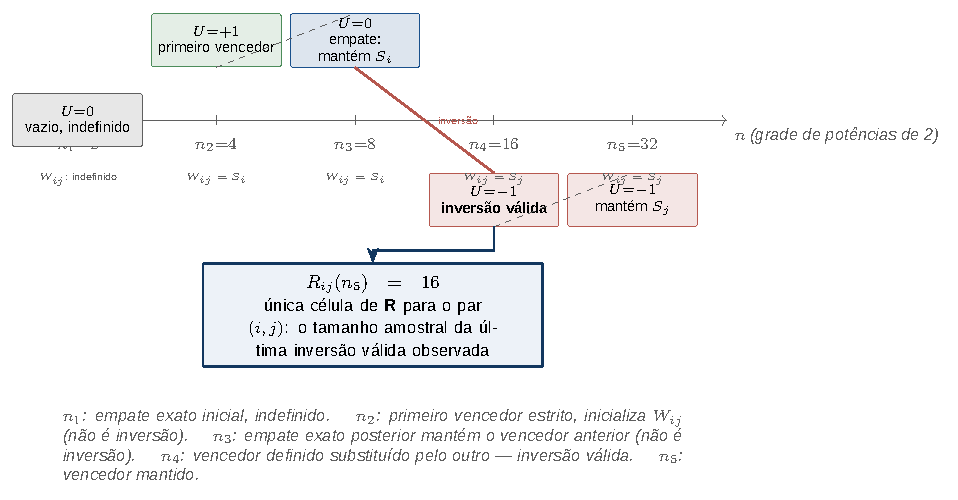
\includegraphics[width=0.85\textwidth]{figures/conceptual/trajetoria_vencedor.pdf}
  \sourcebelow{elaboração própria}
  \notailustracao{Exemplo esquemático; não corresponde a um par específico de nenhum dataset}
\end{figure}

O objeto formal precisa armazenar somente as $q(q-1)/2$ comparações não ordenadas, $\mathcal{P}=\{(i,j):1\leq i<j\leq q\}$, porque $W_{ji}=-W_{ij}$ fora dos casos indefinidos (justificativa completa no Apêndice~D). A matriz quadrada mostrada nos relatórios duplica essas relações para facilitar a leitura visual: a diagonal é vazia, um triângulo determina o outro e as cores identificam qual elemento do par possui menor perda. A Figura~\ref{fig:occupancy-winner-matrices} do Capítulo~5 ilustra, com dados reais do cenário Occupancy Detection, como esse resultado par a par se reorganiza entre $n=2$ e $n=512$.

Essa representação contém muito mais informação do que a identidade do primeiro colocado. Se o vencedor absoluto muda por uma diferença residual, a maioria das relações entre alternativas pode continuar preservada. Para decisões de custo, interessa saber se um subconjunto mais barato permanece superior a numerosas alternativas, não apenas se ocupa exatamente a primeira linha do ranking.

\section{\WinnersAgreement}
\label{sec:winner-agreement}

A \WinnersAgreement{} ($\AW$) compara as relações efetivas de vencedor do braço sintético com as do braço real, usando $\Wmat$ --- e não o resultado observado $U$ --- de modo que um empate exato posterior não é tratado como perda de informação. Pares em que $\Wmat$ permanece indefinido em qualquer um dos braços são ignorados, pois não apresentam um vencedor efetivo comparável. Seja
\begin{equation}
  \mathcal{P}_{\mathrm{valid}}^{(g,f)}(n)
  =\left\{(i,j)\in\mathcal{P}:
  W^{(R,f)}_{ij}(n)\neq0\;\land\;
  W^{(g,f)}_{ij}(n)\neq0\right\}.
\end{equation}
A métrica é
\begin{equation}
  \AW^{(g,f)}(n)=
  \frac{
    \displaystyle\sum_{(i,j)\in\mathcal{P}_{\mathrm{valid}}^{(g,f)}(n)}
    \mathbf{1}\!\left\{W^{(R,f)}_{ij}(n)=W^{(g,f)}_{ij}(n)\right\}
  }{
    \left|\mathcal{P}_{\mathrm{valid}}^{(g,f)}(n)\right|
  }.
  \label{eq:winners-agreement}
\end{equation}
Se não houver pares válidos, o valor é reportado como indisponível. Além da proporção, os relatórios registram o número total de pares, pares válidos, concordantes e ignorados por indefinição. A autocorrelação do braço real é 1 quando há pares comparáveis.

\section{Inversões de superioridade preditiva e matriz de inversões \texorpdfstring{$\Rmat$}{R}}
\label{sec:reversal-matrix}

A relação efetiva de vencedor $\Wmat$ descreve quem vence em cada $n$, mas não descreve, por si só, quando essa relação mudou. Uma \textbf{\PairwiseSuperiorityReversal{}} (\WinnerReversal{}) ocorre em $n_k$, $k\geq2$, exatamente quando um vencedor efetivo já definido é substituído pelo outro elemento do par:
\begin{equation}
  W^{(g,f)}_{ij}(n_{k-1})\neq0,\qquad
  W^{(g,f)}_{ij}(n_k)\neq0,\qquad
  W^{(g,f)}_{ij}(n_k)\neq W^{(g,f)}_{ij}(n_{k-1}).
  \label{eq:valid-reversal}
\end{equation}
Não constituem inversão: um empate inicial; empates iniciais repetidos; o aparecimento do primeiro vencedor estrito; um empate posterior, que apenas mantém o vencedor anterior; ou a simples aproximação das curvas sem troca do vencedor efetivo.

Para o prefixo terminado em $n_t$, a \textbf{matriz de inversões} armazena, para cada par, apenas o tamanho amostral da inversão válida mais recente:
\begin{equation}
  R^{(g,f)}_{ij}(n_t)=
  \begin{cases}
    \max\mathcal{E}^{(g,f)}_{ij}(n_t), & \mathcal{E}^{(g,f)}_{ij}(n_t)\neq\varnothing,\\
    \varnothing, & \mathcal{E}^{(g,f)}_{ij}(n_t)=\varnothing,
  \end{cases}
  \label{eq:reversal-matrix}
\end{equation}
em que $\mathcal{E}^{(g,f)}_{ij}(n_t)$ é o conjunto de tamanhos amostrais do prefixo em que o par $(i,j)$ sofreu inversão válida (definição completa no Apêndice~D).

\begin{definitionbox}[Regra de existência de $R_{ij}$]
A célula $R_{ij}(n_t)$ existe \textbf{se e somente se} o par $(i,j)$ sofreu ao menos uma inversão válida de vencedor no prefixo avaliado. Ela não existe apenas porque um subconjunto vence desde o primeiro ponto da grade, apenas porque o primeiro vencedor aparece depois de empates iniciais, apenas porque as curvas se aproximam, ou apenas porque um subconjunto permanece vencedor durante todo o prefixo.
\end{definitionbox}

Diferentemente de $\Wmat$, a matriz $\Rmat$ não é antissimétrica: ela armazena um único valor por par não ordenado, no triângulo superior ($i<j$); a diagonal e o triângulo inferior são indisponíveis, e $\Rmat$ não guarda separadamente qual subconjunto passou a vencer após a inversão --- essa informação é recuperável diretamente em $\Wmat(n_t)$. O Apêndice~D reproduz, para o cenário SUPPORT2 (Random Forest, execução \textit{full}, $n\leq512$), as matrizes $\Wmat$ e $\Rmat$ completas de sete subconjuntos de referência lado a lado para os braços \RealToReal{} e \GaussianToReal.

\section{Concordância de existência de inversões}
\label{sec:ar}

Para o braço $g$ e o prefixo $n_t$, o \textbf{suporte de inversões} é o conjunto de pares não ordenados com $\Rmat$ definida:
\begin{equation}
  \ReversalSupport_g(n_t)=\{(i,j):i<j,\;R^{(g,f)}_{ij}(n_t)\neq\varnothing\}.
\end{equation}
A \ReversalExistenceAgreement{} compara o suporte do braço sintético com o suporte do braço real por concordância de Jaccard:
\begin{equation}
  \AR(n_t)=
  \frac{|\ReversalSupport_{\mathrm{real}}(n_t)\cap\ReversalSupport_g(n_t)|}
       {|\ReversalSupport_{\mathrm{real}}(n_t)\cup\ReversalSupport_g(n_t)|}.
  \label{eq:ar}
\end{equation}
Convenções: no primeiro prefixo, $\AR$ é indisponível, pois nenhuma inversão pode ainda ter ocorrido; se a união dos suportes for vazia em um prefixo posterior, $\AR=1$, com o status explícito \emph{sem inversões em nenhum braço} --- essa concordância é sobre a \emph{ausência} de inversões, não sobre coincidência de posições; se a união for não vazia e a interseção for vazia, $\AR=0$; caso contrário, aplica-se o Jaccard usual.

\section{Distância e similaridade dos tamanhos amostrais das inversões}
\label{sec:sr}

Para os pares em que ambos os braços sofreram inversão --- o \textbf{suporte compartilhado} $\SharedReversalSupport(n_t)=\ReversalSupport_{\mathrm{real}}(n_t)\cap\ReversalSupport_g(n_t)$ --- é possível perguntar se as inversões mais recentes ocorreram em tamanhos amostrais semelhantes. A \MeanLogReversalDistance{} é
\begin{equation}
  \DR(n_t)=
  \frac{1}{|\SharedReversalSupport(n_t)|}
  \sum_{(i,j)\in\SharedReversalSupport(n_t)}
  \left|
    \log_2 R^{(g,f)}_{ij}(n_t)-\log_2 R^{(\mathrm{real},f)}_{ij}(n_t)
  \right|,
  \label{eq:dr}
\end{equation}
medida em níveis da grade de potências de dois. A \ReversalSampleSizeSimilarity{} normaliza essa distância pela amplitude logarítmica do prefixo:
\begin{equation}
  \SR(n_t)=
  \operatorname{clip}_{[0,1]}
  \left(
    1-\frac{\DR(n_t)}{\log_2 n_t-\log_2 n_1}
  \right).
  \label{eq:sr}
\end{equation}
Convenções: no primeiro prefixo, $\SR$ é indisponível; se não há pares no suporte compartilhado, $\SR$ é indisponível --- inclusive quando $\ReversalSupport_{\mathrm{real}}(n_t)=\ReversalSupport_g(n_t)=\varnothing$, caso em que $\AR=1$ mas $\SR$ permanece indisponível, porque não há nenhum tamanho amostral de inversão para comparar; tamanhos amostrais compartilhados idênticos produzem $\SR=1$.

\begin{interpretationbox}
$\AR$ e $\SR$ respondem perguntas diferentes e nunca são combinados em um produto ou índice único. $\AR$ pergunta se os \emph{mesmos pares} sofrem inversão; $\SR$, condicional a $\AR$ ter identificado pares compartilhados, pergunta se essas inversões ocorrem em \emph{regimes amostrais semelhantes}. Um valor de $\AR=1$ obtido por ausência simultânea de inversões (status \emph{sem inversões em nenhum braço}) não implica nenhuma informação sobre tamanhos amostrais, porque não há inversões cujos tamanhos possam ser comparados.
\end{interpretationbox}

A Figura~\ref{fig:construcao-ar-sr} esquematiza a construção progressiva de $\AR$ e $\SR$ ao longo de prefixos crescentes da grade amostral.

\begin{figure}[H]
  \centering
  \caption{Construção separada de $A_R$ e $S_R$ em prefixos crescentes da grade amostral}
  \label{fig:construcao-ar-sr}
  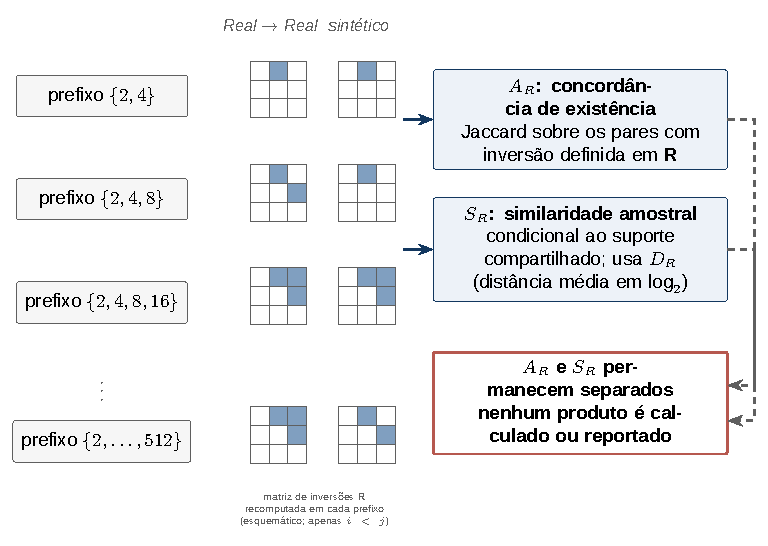
\includegraphics[width=0.86\textwidth]{figures/conceptual/construcao_ar_sr.pdf}
  \sourcebelow{elaboração própria}
  \notailustracao{A cada prefixo, a matriz de inversões $\mathbf{R}$ é recomputada para os braços real e sintético; $A_R$ e $S_R$ são calculados separadamente a partir dela e nunca combinados}
\end{figure}

\section{Leitura integrada do perfil}

Os quatro indicadores respondem a perguntas diferentes: a \textbf{correlação de ranking} ($\rankrho$) pergunta se a ordenação global dos subconjuntos é semelhante, tolerando pequenas trocas locais; a \textbf{\WinnersAgreement{}} ($\AW$) mede quantas relações efetivas de vencedor par a par são preservadas, e pode apoiar comparações de eficiência entre muitas alternativas; a \textbf{\ReversalExistenceAgreement{}} ($\AR$) pergunta se os mesmos pares sofrem ao menos uma inversão de vencedor, indiferente ao tamanho amostral em que ela ocorreu; e a \textbf{\ReversalSampleSizeSimilarity{}} ($\SR$), condicional ao suporte compartilhado de inversões, pergunta se essas inversões ocorrem em regimes amostrais semelhantes.

Nenhum indicador é reduzido à identidade da primeira posição, e nenhum indicador subsume os demais. A coincidência do melhor subconjunto pode ser relatada como consequência do ranking, mas um erro mínimo entre alternativas quase empatadas não deve dominar a avaliação. Para planejamento de custos, $\rankrho$ e $\AW$ são particularmente úteis porque revelam a organização global e as relações efetivas entre configurações; $\AR$ e $\SR$ acrescentam quando e onde essa organização muda à medida que mais rótulos se tornam disponíveis --- sem, no entanto, serem combinados entre si.

A preservação do perfil de cooperação preditiva é, portanto, multidimensional. Um braço pode apresentar ranking alto, elevada \WinnersAgreement{} e $\AR$ moderado; ou pode preservar os pares de inversão sem preservar os tamanhos amostrais em que ocorrem. O relatório mantém os quatro indicadores separados para que essas combinações permaneçam visíveis, em vez de ocultá-las em um índice único --- como o Capítulo~5 demonstra com dados reais dos quatro cenários de escala completa.
